\section{Marco teórico}
Además de presentar la teoría relacionada con el MLP es necesario explicar lo que es el algoritmo de propagación hacia atrás (o Backpropagation en inglés) que es la base del aprendizaje de esta arquitectura.

El perceptrón multicapa (Multilayer Perceptron) surge de la necesidad de tratar problemas que no son linealmente separables es por esto que Frank Rosenblatt y Bernard Widrow propusieron redes multicapa pero no pudieron generalizar los algoritmos necesarios para entrenar dichas redes.

Dicho algoritmo fue descrito hasta 1974 por Paul Werbos pero fue hasta 1980 cuando se empezó a divulgar y fue entonces cuando el MLP entrenado por el algoritmo de backpropagation se ha convertido en la red neuronal más utilizado. \cite{libro1}
\subsection{Perceptron multicapa}
Un perceptron multicapa es aquello en el cual la salida de una capa es la entrada de la siguiente capa, un ejemplo de esto es el mostrado en la figura \ref{fig:MLP} donde se presenta un MLP de tres capas. En un MLP cada capa puede tener diferente número de neuronas y distintas funciones de transferencia. Para poder diferenciar cada capa se utiliza un superindice como por ejemplo:
\[ \begin{bmatrix} R & S^1 & S^2 & S^3 & \dots & S^N \end{bmatrix} \]

\begin{figure}[H]
    \begin{center}
        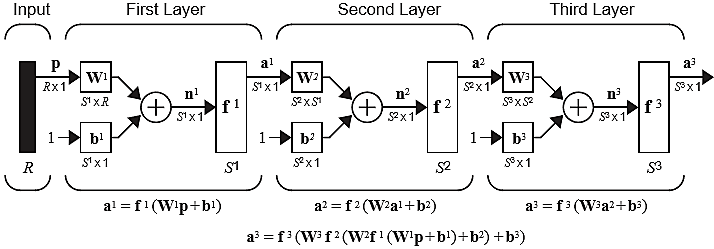
\includegraphics[width=16cm]{img/MLP.png}
        \caption{Perceptron de tres capas. \cite{libro1}}
        \label{fig:MLP}
    \end{center}
\end{figure}

En donde $S^1$ indica el número de neuronas de la capa uno, $S^2$ el número de neuronas en la capa dos y así consecutivamente. Esta misma estructura permite identificar la arquitectura de la red neuronal donde $R$ es el número de entradas. Para identificar el conjunto de funciones que se utiliza en cada capa se utiliza.

\[ \begin{bmatrix} F^1 & F^2 & F^3 & \dots & F^N \end{bmatrix} \]


Cada uno de estos elementos hace referencia alguna función de activación, las funciones que más se suelen utilizar son no lineales algunas de estas son.

\begin{itemize}
    \item Log-Sigmoid
    \[ a = \dfrac{1}{1+e^{-n}}\]
    \item Hyperbolic Tangent Sigmoid
    \[ a = \dfrac{e^n - e^{-n}}{e^n + e^{-n}}\]
    \item Linear
    \[ a = n\]
\end{itemize}

\begin{figure}[H]
    \begin{center}
        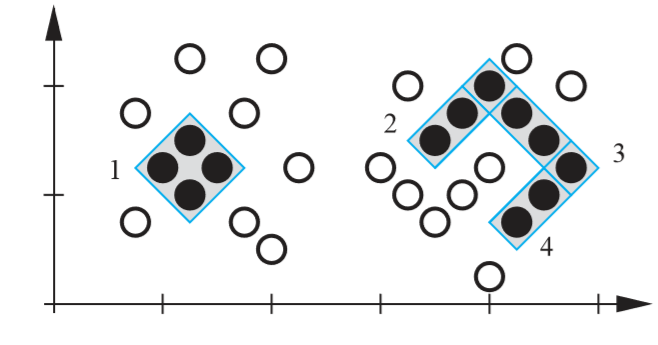
\includegraphics[width=7cm]{img/patrones.png}
        \caption{Clasificación de patrones. \cite{libro1}}
        \label{fig:clasificacion}
    \end{center}
\end{figure}

Las principales aplicaciones del MLP son:
\begin{itemize}
    \item Clasificación de patrones, objetos y caracteres como en la figura \ref{fig:clasificacion}.
    \item Aproximación de funciones.
    \item Compresión y codificación de información
    \item Reconocimiento de palabras (véase figura \ref{fig:palabras}).
    \item Segmentación de imágenes \cite{pdf}.
\end{itemize}

\begin{figure}[H]
    \begin{center}
        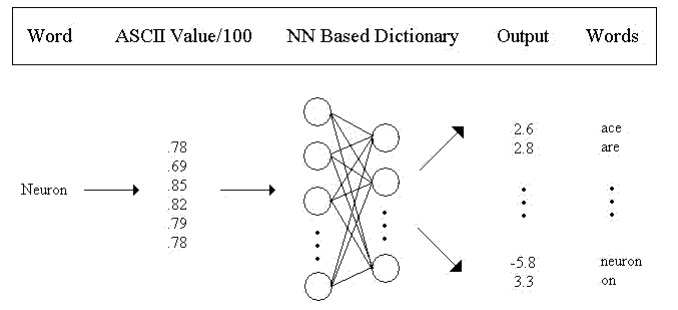
\includegraphics[width=12cm]{img/palabras.png}
        \caption{Diagrama del reconocimiento de palabras. \cite{pdf}}
        \label{fig:palabras}
    \end{center}
\end{figure}

La aproximación de señales se usa en sistemas de control en donde se trata de encontrar una función que pueda mapear mediciones de salidas a controles de entrada. Se puede realizar la aproximación de cualquier función si se tienen suficientes neuronas en las capas ocultas. 
\subsection{Backpropagation}
Para el estudio de backpropagation es importante conocer las ecuaciones que se usan en el aprendizaje que realiza. La primera de ellas está relacionada con las salidas de cada capa del MLP, estas ecuaciones son otra forma de representar la arquitectura de la figura \ref{fig:MLP}.

\begin{equation} \label{eq:1}
\boldsymbol{a}^0 = \boldsymbol{p}
\end{equation}
\begin{equation} \label{eq:2}
\boldsymbol{a}^{m+1} = \boldsymbol{f}^{m+1}(\boldsymbol{W}^{m+1}\boldsymbol{a}^{m}+\boldsymbol{b}^{m+1}
), \quad \text{Para $m=0, 1, \ldots M-1$}
\end{equation}
\begin{equation} \label{eq:3}
    \boldsymbol{a} = \boldsymbol{a}^{M}
\end{equation}
El valor de $M$ es el número de capas que tiene la red. La ecuación \ref{eq:1} hace referencia a que la capa uno tiene como entrada el conjunto de datos $\boldsymbol{p}$. Por otro lado la ecuación \ref{eq:3} es considerado como la salida final de la red neuronal.

El algoritmo backpropagation es una generalización del algoritmo LMS ya que ambos utilizan el error cuadrático medio, además utiliza un conjunto de entrenamiento compuesto por la entrada a la red y su correspondiente salida objetivo.
\[ \left\lbrace \boldsymbol{p_1}, \boldsymbol{t_1} \right\rbrace, \left\lbrace \boldsymbol{p_2}, \boldsymbol{t_2} \right\rbrace, \dots, \left\lbrace \boldsymbol{p_Q}, \boldsymbol{t_Q} \right\rbrace  \]
El objetivo de utilizar el una entrada y un target es utilizar un algoritmo de aprendizaje y con ello minimizar el error de salida de la red, dicho error es calculado con la siguiente formula.
\[ F(\boldsymbol{x}) = E \left[ \boldsymbol{e}^{T}\boldsymbol{e} \right] = E \left[ (\boldsymbol{t-a})^{T}(\boldsymbol{t-a}) \right]  \]
Aquí, $\boldsymbol{x}$ es el vector de pesos y bias de la red. Para una iteración (la propagación de un dato) esta ecuación se convierte en.
\[ \hat{F} (\boldsymbol{x}) = E \left[ \boldsymbol{e}^{T}\boldsymbol{e} \right] = E \left[ (\boldsymbol{t-a})^{T}(\boldsymbol{t-a}) \right]  \]
Esto hace que el algoritmo de gradiente descendente para pesos y bias sea.
\begin{equation} \label{eq:4}
w_{i, j}^{m}(k+1) = w_{i, j}^{m}(k) - \alpha \frac{\partial \hat{F}}{\partial w_{i, j}^{m}}
\end{equation}

\begin{equation} \label{eq:5}
b_{i}^{m}(k+1) = b_{i}^{m}(k) - \alpha \frac{\partial \hat{F}}{\partial b_{i}^{m}}
\end{equation}

Para poder trabajar con estas ecuaciones se debe de utilizar la regla de la cadena para facilitar el calculo de las derivadas parciales. Esto produce que se definan nuevos elementos los cuales son las sensitividades de $\hat{F}$ para cada elemento en cada capa de la red, dichas sensitividades producen los siguientes cambios.
\begin{equation} \label{eq:6}
\frac{\partial \hat{F}}{\partial w_{i, j}^{m}} = s_{i}^{m}a_{j}^{m-1}
\end{equation}
\begin{equation} \label{eq:7}
\frac{\partial \hat{F}}{\partial b_{i}^{m}} = s_{i}^{m}
\end{equation}
Al remplazar \ref{eq:6} y \ref{eq:7} en las ecuaciones \ref{eq:4} y \ref{eq:5} respectivamente y generalizando dichas ecuaciones a toda la matriz de pesos y bias para cada capa obtenemos las siguientes expresiones.

\begin{equation} \label{eq:8}
\boldsymbol{W}^{m}(k+1) = \boldsymbol{W}^{m}(k) - \alpha \boldsymbol{s}^{m} (\boldsymbol{a}^{m-1})^T
\end{equation}

\begin{equation} \label{eq:9}
\boldsymbol{b}^{m}(k+1) = \boldsymbol{b}^{m}(k) - \alpha \boldsymbol{s}^{m}
\end{equation}
Ahora lo importante es definir $\boldsymbol{s}^{m}$ para cada capa $\boldsymbol{m}$ de la red neuronal. Para la ultima capa del perceptrón, la capa $\boldsymbol{M}$ la sensitividad queda definida como:
\begin{equation} \label{eq:10}
    \boldsymbol{s^M} = 
    -2\boldsymbol{\dot{F}^{M}}(\boldsymbol{n^{M}})(\boldsymbol{t-a})
\end{equation}
Mientras que para el resto de las capas la sensitividad es:
\begin{align*}
\boldsymbol{s}^M &= 
-2\boldsymbol{\dot{F}}^{M}(\boldsymbol{n}^{M})(\boldsymbol{t-a}) \\
\boldsymbol{s}^{m} &= 
\boldsymbol{\dot{F}}^{m}(\boldsymbol{n}^{m})(\boldsymbol{W}^{m+1})^{T}
\boldsymbol{s}^{m+1} & & \text{para $m=M-1, \ldots, 2, 1$} \\
\text{donde} \\
\boldsymbol{\dot{F}}^{m}(\boldsymbol{n}^{m}) &=
\begin{bmatrix}
\dot{f}^{m}(n_{1}^{m}) & 0 & \ldots & 0 \\
0 & \dot{f}^{m}(n_{2}^{m}) & \ldots & 0 \\
\vdots & \vdots & \ddots & \vdots \\
0 & 0 & \ldots & \dot{f}^{m}(n_{s^{m}}^{m})
\end{bmatrix} \\
\dot{f}^{m}(n_{j}^{m}) &= 
\frac{\partial \dot{f}^{m}(n_{j}^{m})}{\partial n_{j}^{m}}
\end{align*}
Finalmente la actualización de pesos y bias en cada iteración queda definido por las siguientes ecuaciones
\begin{align*}
\boldsymbol{W}^{m}(k+1) &= \boldsymbol{W}^{m}(k)-\alpha 
\boldsymbol{s}^{m}(\boldsymbol{a}^{m-1})^{T}, \\
\boldsymbol{b}^{m}(k+1) &= \boldsymbol{b}^{m}(k) - \alpha \boldsymbol{s}^{m}
\end{align*}